\subsection{Application: Edge Artificial Intelligence for Industrial Internet of Things}

Edge-AI deployment is a useful Foundations application because it forces a model-selection problem to include resource constraints rather than predictive accuracy alone. A model intended for a microcontroller, embedded gateway, or industrial sensor node must fit within memory and latency budgets while preserving enough predictive quality for the operational decision. Compression therefore changes the hypothesis representation and the deployment objective at the same time.

Quantization is one of the simplest ways to make that tradeoff explicit. Reducing weight precision decreases storage and can improve arithmetic efficiency on suitable hardware, but it also perturbs the learned parameter vector. Whether the perturbation is acceptable must be validated on held-out data rather than inferred from bit width alone. This connects directly to the chapter's themes of regularization, model selection, validation, and deployment-aware objectives.

The controlled experiment below uses a standardized logistic-regression classifier on the Wisconsin Diagnostic Breast Cancer dataset. The model is intentionally small so that the numerical consequences of weight-only symmetric quantization are transparent. The experiment is not a hardware benchmark; it isolates the storage-versus-prediction tradeoff that a deployment pipeline must evaluate before device-specific latency and energy measurements are added.

\textbf{Problem}

The task is to reduce model storage while preserving held-out discrimination and classification performance. The engineering question is not simply whether lower-bit weights are possible, but how much predictive behavior changes as the representation becomes more compressed.

\textbf{Dataset}

The benchmark uses the scikit-learn Wisconsin Diagnostic Breast Cancer dataset with a stratified 70/30 train-test split and random seed 1729. Continuous features are standardized using statistics fit only on the training partition. The held-out test partition is used for the final accuracy, ROC--AUC, and log-loss comparison.

\textbf{Model}

A logistic-regression classifier is trained in floating-point precision. The learned coefficient vector is then quantized with symmetric per-tensor quantization to 8, 4, 3, and 2 bits per weight. The intercept remains in floating point so the experiment isolates the effect of coefficient quantization. The packed storage values are theoretical coefficient-storage requirements rather than measurements of a particular file format or processor runtime.

\textbf{Method}

For each target bit width, the coefficient vector is scaled to the signed quantization range, rounded, clipped, and dequantized back to floating point for inference. The same held-out observations are scored with every representation. Because the decision boundary changes slightly after quantization, the comparison reports ranking and probability-sensitive metrics in addition to thresholded accuracy.

\textbf{Evaluation}

Figure~\ref{fig:ch1-edge-quantization} reports both resource and predictive effects. Panel (a) shows theoretical packed coefficient storage as precision decreases from float64 to 2-bit weights. Panel (b) shows held-out accuracy and ROC--AUC for the same representations. Table~\ref{tab:ch1-edge-quantization} reports the numerical comparison, including log loss.

\begin{figure}[t]
\centering
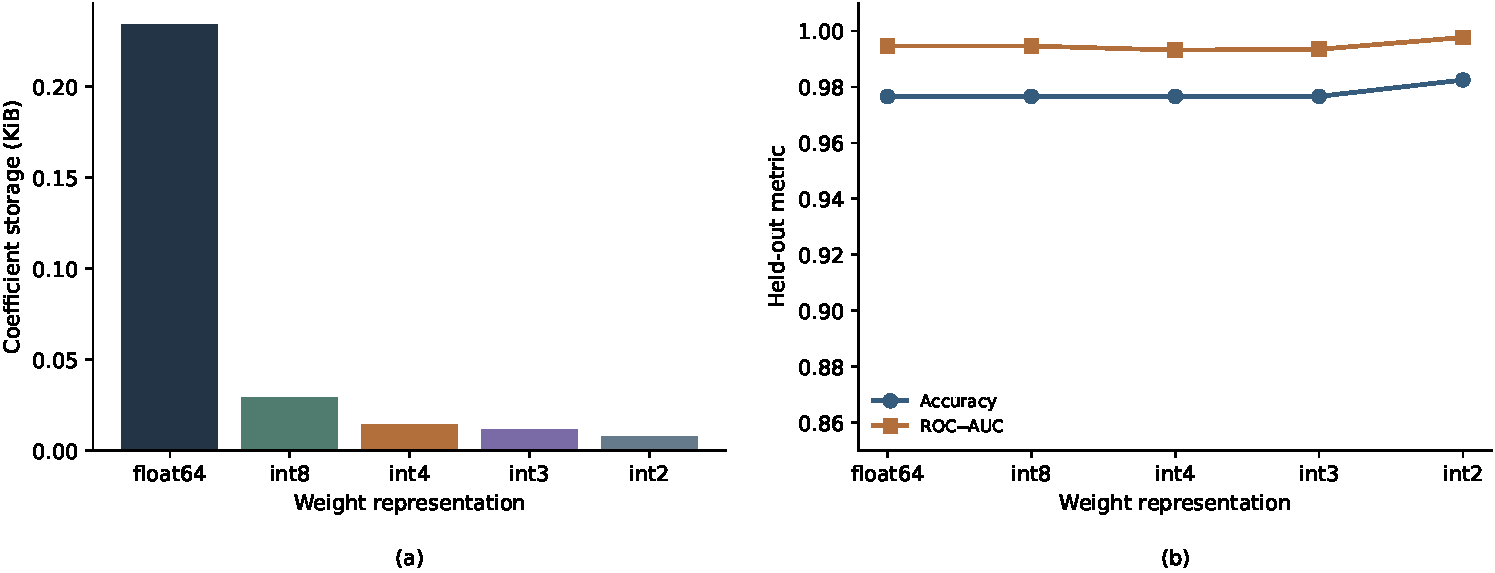
\includegraphics[width=\BookFigureWidth]{figures/ch01_edge_quantization_tradeoff.pdf}
\caption{Controlled model-compression benchmark on the Wisconsin Diagnostic Breast Cancer dataset. (a) Theoretical packed storage for the logistic-regression coefficient vector under floating-point and symmetric low-bit weight representations. (b) Held-out accuracy and ROC--AUC for the corresponding dequantized models. The experiment isolates weight-representation effects and does not claim device-specific latency or energy savings, which require measurements on the target hardware.}
\label{fig:ch1-edge-quantization}
\end{figure}

\begin{table}[t]
\centering
\small
\caption{Reproduced weight-quantization comparison for the standardized logistic-regression model. Storage is the theoretical packed coefficient storage, not serialized model size.}
\label{tab:ch1-edge-quantization}
\begin{tabular}{lrrrr}
\toprule
Representation & Storage (bytes) & Accuracy & ROC--AUC & Log loss \\
\midrule
float64 & 240 & 0.9766 & 0.9946 & 0.0824 \\
int8 & 30 & 0.9766 & 0.9946 & 0.0824 \\
int4 & 15 & 0.9766 & 0.9931 & 0.0843 \\
int3 & 12 & 0.9766 & 0.9934 & 0.0796 \\
int2 & 8 & 0.9825 & 0.9977 & 0.0561 \\
\bottomrule
\end{tabular}
\end{table}

\textbf{Results}

The 8-bit representation reduces theoretical coefficient storage by a factor of eight while leaving the reported accuracy and ROC--AUC unchanged to four decimal places in this split. More aggressive quantization also remains competitive. The 2-bit result is slightly stronger on this particular holdout set, which should be interpreted as a split-specific perturbation or regularization effect rather than evidence that 2-bit weights are universally superior. The important engineering conclusion is that compression must be validated empirically instead of assumed to produce a monotonic accuracy penalty.

\textbf{Error Analysis}

Quantization errors should be examined at the prediction level, especially for observations close to the original decision boundary. A representation can preserve aggregate accuracy while changing which specific cases are misclassified or altering probability calibration. For safety- or cost-sensitive deployment, disagreement analysis between the reference and compressed model is therefore as important as the aggregate accuracy difference.

\textbf{Limitations}

This experiment uses a very small linear model and theoretical packed weight storage. It does not include activation quantization, integer arithmetic kernels, operator support, memory alignment, runtime overhead, compiler effects, latency, or energy measurements. The dataset is also unrelated to a specific industrial IoT sensor workload. The benchmark is intentionally a Foundations demonstration of compression-aware model validation rather than a complete embedded-system evaluation.

\textbf{Deployment / Engineering Implications}

A deployment decision should combine predictive metrics with measured memory, latency, throughput, and energy on the target device. Quantization should be treated as a new model configuration that requires its own validation, calibration checks, and rollback criteria. This extends the chapter's model-selection framework: the preferred model is the one that satisfies the operational objective under explicit resource constraints, not necessarily the model with the highest unconstrained floating-point score.
